\documentclass[11pt,a4paper]{article}
\usepackage[utf8]{inputenc}\usepackage[T1]{fontenc}\usepackage{lmodern}\usepackage[a4paper,margin=2.6cm]{geometry}
\usepackage{amsmath,amssymb,amsfonts,bm,mathtools,booktabs,array,graphicx,pgfplots,hyperref,xcolor,microtype}
\pgfplotsset{compat=1.18}
\hypersetup{colorlinks=true,linkcolor=blue!60!black,citecolor=blue!60!black,urlcolor=blue!60!black}
\newcommand{\Tr}{\operatorname{Tr}}\newcommand{\Lent}{L_{\rm ent}}\newcommand{\DR}{\Delta_R^{\rm flow}}
\title{\textbf{Paper 28 --- Modular Time and Mutual-Information Geometry}\\[0.35em]\large Frozen TFIM Benchmarks from $N=6$ to $N=10$}
\author{Farid Hamdad\\\small Bottom-Up Quantum Gravity Program}\date{2026}
\begin{document}\maketitle
\begin{abstract}
Bottom-Up Quantum Gravity (BuP) assigns distinct roles to information geometry and modular dynamics. Spatial structure is encoded by the mutual-information graph $W_{ij}=I(i:j)$, while intrinsic relational evolution of a reduced subsystem $A$ is generated by its modular Hamiltonian $K_A=-\log\rho_A$. This paper tests whether those two sectors are dynamically compatible in finite transverse-field Ising models. For $N=6,8,10$, we prepare a time-reversal mixed state using a frozen Strang-splitting protocol, compute $W$ inside a prefix subsystem $A$, normalize $K_A$, and measure operator spreading through a Pauli-averaged squared commutator $C_{ij}(\tau)$. In all four frozen primary arms---$N6/A3$, $N8/A4$, $N10/A4$, and $N10/A5$---the residual contrast $\DR=R(G_{\rm chain})-R(W)$ is positive. On 1023 nonzero frozen modular times, $W$ has the lower residual on $99.3157\%$, $99.1202\%$, $99.2180\%$, and $100\%$ of points, respectively. The fixed-subsystem control $N8/A4\to N10/A4$ changes the mean secondary contrast only from $0.0687091$ to $0.0699113$. The result supports finite-system compatibility between modular dynamics and mutual-information geometry, not a continuum, causal, Einstein, or universality theorem.
\end{abstract}
\tableofcontents
\section{Introduction}
BuP separates a spatial information sector from an intrinsic modular-dynamics sector. The spatial candidate begins from $W_{ij}=I(i:j)$; the temporal candidate begins from $\rho_A$ and $K_A=-\log\rho_A$. These objects are not identical: $W$ is pairwise, while $K_A$ is a many-body operator. The test is therefore operational: does operator spreading generated by $K_A$ follow $W$ more closely than the bare microscopic graph?
\section{Spatial and temporal sectors}
For $I(i:j)=S(\rho_i)+S(\rho_j)-S(\rho_{ij})$, BuP sets $W_{ij}=I(i:j)$ and $\Lent=D-W$. A compatible information distance is $d_{ij}^{\rm ent}=-\log[I(i:j)/(I_{\max}+\epsilon)]$. For the same subsystem, $K_A=-\log\rho_A$ and $O(\tau)=e^{iK_A\tau}Oe^{-iK_A\tau}$. Since $[K_A,\rho_A]=0$, the nontrivial test acts on observables rather than evolving $\rho_A$ by its own modular generator.
\section{Frozen TFIM benchmark}
We use $H=-J\sum_{i=0}^{N-2}Z_iZ_{i+1}-h\sum_{i=0}^{N-1}X_i$ with $J=h=1$, initial $|+\rangle^{\otimes N}$, and six Strang steps of $\Delta t=0.35$. The analysis state is the time-reversal mixture $\rho_{\rm TR}=\tfrac12[|\Psi(+t)\rangle\langle\Psi(+t)|+|\Psi(-t)\rangle\langle\Psi(-t)|]$ with nominal $t=2.1$.

For strictly positive eigenvalues $\lambda_n$ of $\rho_A$, write $\kappa_n=-\log\lambda_n$ and normalize
\[
\widetilde K_A=\frac{K_A-\langle\kappa\rangle I}{\operatorname{std}(\kappa)}.
\]
No regularization is used when the frozen positivity gate $\lambda_{\min}>0$ passes.

For $i\ne j$,
\[
C_{ij}(\tau)=\frac19\sum_{a,b=X,Y,Z}\Tr\!\left[\rho_A[\sigma_i^a(\tau),\sigma_j^b]^\dagger[\sigma_i^a(\tau),\sigma_j^b]\right],
\]
with $\sigma_i^a(\tau)=e^{i\widetilde K_A\tau}\sigma_i^ae^{-i\widetilde K_A\tau}$. At short time, $C_{ij}(\tau)=A_{ij}\tau^2+\cdots$ and $v_{ij}^{\rm mod}=\sqrt{A_{ij}}$.
\section{Comparator metric}
For profile $v$ and comparator $g$,
\[
c(g)=\max\!\left(0,\frac{v\cdot g}{g\cdot g}\right),\qquad R(g)=\frac{\|v-c(g)g\|}{\|v\|},
\]
and
\[
\boxed{\DR=R(G_{\rm chain})-R(W)}.
\]
Positive $\DR$ favors $W$ descriptively.
\section{Primary results}
\begin{table}[ht]\centering\caption{Primary short-time modular-flow comparison.}\begin{tabular}{lrrrr}\toprule Arm & $R_W$ & $R_{\rm chain}$ & $\DR$ & $\lambda_{\min}$\\\midrule
$N6/A3$&0.028472&0.180430&0.151958&$3.706\times10^{-3}$\\
$N8/A4$&0.258436&0.381359&0.122924&$3.181\times10^{-4}$\\
$N10/A4$&0.255410&0.379609&0.124199&$3.142\times10^{-4}$\\
$N10/A5$&0.402236&0.623098&0.220862&$2.674\times10^{-8}$\\\bottomrule\end{tabular}\end{table}
\begin{figure}[ht]\centering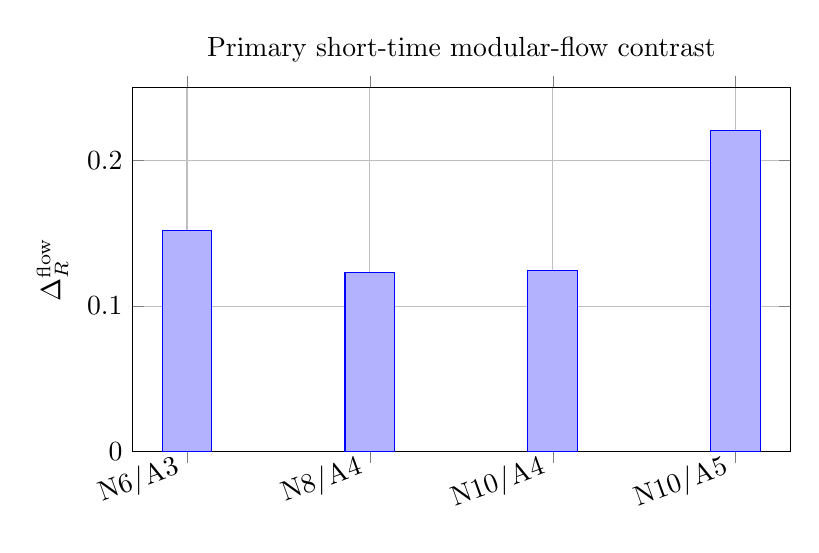
\begin{tikzpicture}
\begin{axis}[
  width=0.82\textwidth,height=6.2cm,
  ybar,bar width=18pt,
  ymin=0,ymax=0.25,
  ylabel={$\Delta_R^{\rm flow}$},
  symbolic x coords={N6/A3,N8/A4,N10/A4,N10/A5},
  xtick=data,
  x tick label style={rotate=20,anchor=east},
  title={Primary short-time modular-flow contrast},
  grid=major
]
\addplot coordinates {(N6/A3,0.1519583896) (N8/A4,0.1229235652) (N10/A4,0.1241991943) (N10/A5,0.2208624919)};
\end{axis}
\end{tikzpicture}
\caption{Primary residual contrast; all frozen arms have $\DR>0$.}\end{figure}
The sign is stable, while magnitude is non-monotonic when $N$ and $|A|$ both change. N10/A5 is positive but strongly conditioned, with condition number about $1.3946\times10^7$.
\section{Secondary frozen-grid dynamics}
The grid is $\tau_k=120k/1023$, $k=0,\ldots,1023$. The zero point is retained in raw curves but excluded from residual metrics; all 1023 nonzero points are retained.
\begin{table}[ht]\centering\caption{Secondary descriptive metrics.}\begin{tabular}{lrrrr}\toprule Arm&$\langle\Delta_R\rangle$&$f(R_W<R_c)$&$\Delta_R^{\min}$&$\Delta_R^{\max}$\\\midrule
$N6/A3$&0.132052&0.993157&-0.030579&0.191262\\
$N8/A4$&0.068709&0.991202&-0.026039&0.225529\\
$N10/A4$&0.069911&0.992180&-0.024641&0.222309\\
$N10/A5$&0.147941&1.000000&0.126910&0.283654\\\bottomrule\end{tabular}\end{table}
\begin{figure}[ht]\centering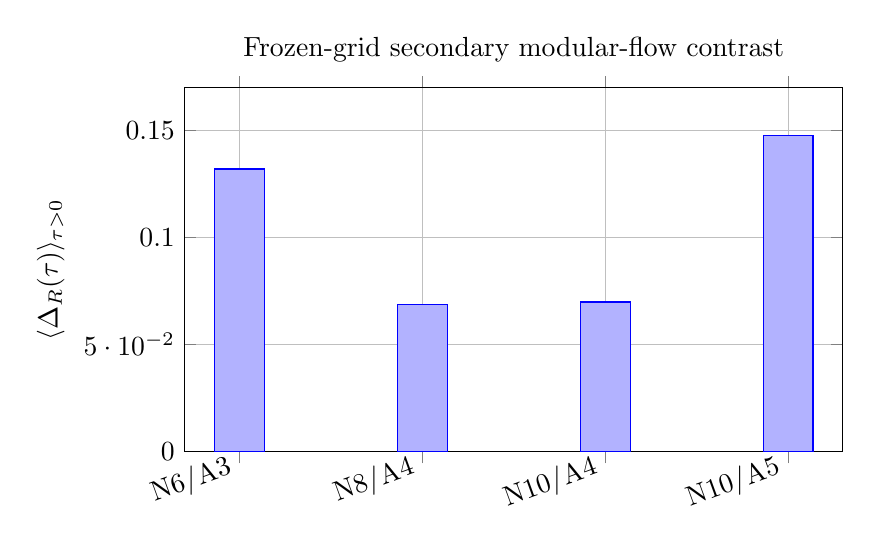
\begin{tikzpicture}
\begin{axis}[
  width=0.82\textwidth,height=6.2cm,
  ybar,bar width=18pt,
  ymin=0,ymax=0.17,
  ylabel={$\langle\Delta_R(\tau)\rangle_{\tau>0}$},
  symbolic x coords={N6/A3,N8/A4,N10/A4,N10/A5},
  xtick=data,
  x tick label style={rotate=20,anchor=east},
  title={Frozen-grid secondary modular-flow contrast},
  grid=major
]
\addplot coordinates {(N6/A3,0.1320520591) (N8/A4,0.0687091263) (N10/A4,0.0699112761) (N10/A5,0.1479409231)};
\end{axis}
\end{tikzpicture}
\caption{Mean contrast on the full nonzero frozen grid.}\end{figure}
For N10/A5, even the minimum is positive, so $W$ has lower residual at every sampled nonzero modular time.
\section{Fixed-subsystem-size control}
At fixed $|A|=4$, primary $\Delta_R$ changes from $0.1229235652$ (N8) to $0.1241991943$ (N10), while mean secondary $\Delta_R$ changes from $0.0687091263$ to $0.0699112761$. The favorable fraction changes from $0.9912023460$ to $0.9921798631$.
\begin{figure}[ht]\centering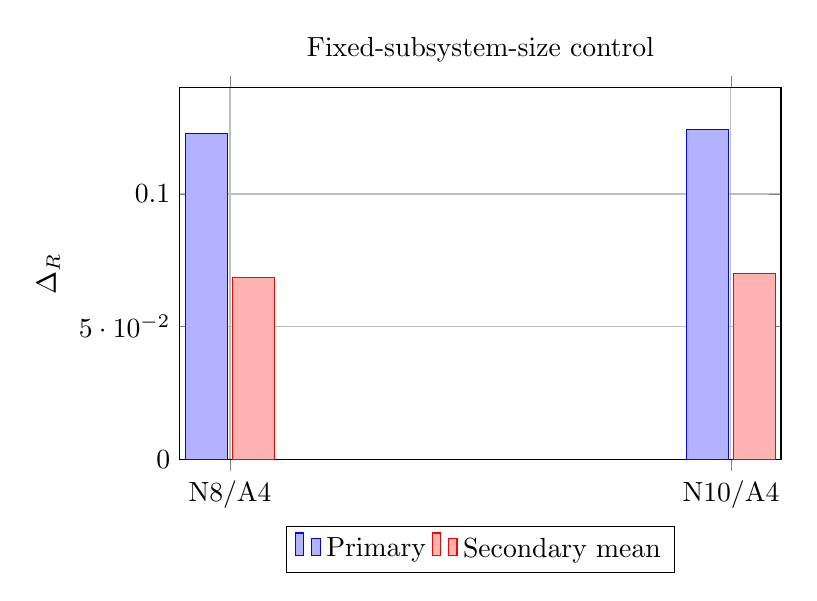
\begin{tikzpicture}
\begin{axis}[
  width=0.76\textwidth,height=6.3cm,
  ybar,bar width=15pt,
  ymin=0,ymax=0.14,
  ylabel={$\Delta_R$},
  symbolic x coords={N8/A4,N10/A4},xtick=data,
  title={Fixed-subsystem-size control},
  legend style={at={(0.5,-0.18)},anchor=north,legend columns=2},
  grid=major
]
\addplot coordinates {(N8/A4,0.1229235652) (N10/A4,0.1241991943)};
\addplot coordinates {(N8/A4,0.0687091263) (N10/A4,0.0699112761)};
\legend{Primary,Secondary mean}
\end{axis}
\end{tikzpicture}
\caption{Fixed-$|A|=4$ control.}\end{figure}
This near-stability indicates that the N10/A5 increase cannot be assigned simply to total system size; the subsystem cut and modular spectrum matter. With only two global sizes at fixed $|A|$, this is descriptive rather than asymptotic evidence.
\section{Dynamical ordering complexity}
The ordering of pairwise $C_{ij}(\tau)$ values changes repeatedly: transition counts are $93,372,365,607$, while distinct observed orderings are $6,221,204,585$ for N6/A3, N8/A4, N10/A4 and N10/A5. Thus the residual advantage is not produced by a static ordering.
\begin{figure}[ht]\centering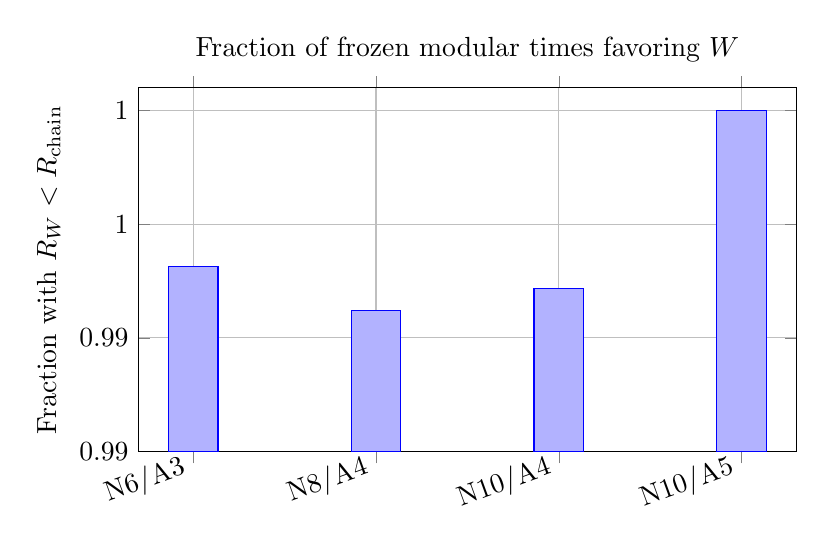
\begin{tikzpicture}
\begin{axis}[
  width=0.82\textwidth,height=6.2cm,
  ybar,bar width=18pt,
  ymin=0.985,ymax=1.001,
  ylabel={Fraction with $R_W<R_{\rm chain}$},
  symbolic x coords={N6/A3,N8/A4,N10/A4,N10/A5},
  xtick=data,
  x tick label style={rotate=20,anchor=east},
  title={Fraction of frozen modular times favoring $W$},
  grid=major
]
\addplot coordinates {(N6/A3,0.9931573803) (N8/A4,0.9912023460) (N10/A4,0.9921798631) (N10/A5,1.0)};
\end{axis}
\end{tikzpicture}
\caption{Fraction of frozen modular times favoring $W$.}\end{figure}
\section{Interpretation for BuP}
The tested chain is
\[
\rho_A\to K_A\to\text{modular operator spreading},
\]
whose pairwise profile is better approximated by $W_{ij}=I(i:j)$ than by bare chain adjacency. This is a compatibility result, not the identity $K_A=W$. It complements earlier BuP spectral compatibility statements such as $K_A\sim f(\Lent)$ by testing operator propagation directly.
\section{Relation to modular theory}
Modular flow is a standard structure in operator-algebraic quantum theory. Tomita--Takesaki theory associates a modular automorphism with a state and algebra, and Bisognano--Wichmann connects modular flow to Lorentz boosts in a Rindler wedge. The present finite-dimensional benchmark assumes neither AQFT nor AdS/CFT; it asks only which candidate graph better organizes state-derived modular spreading.
\section{Limitations}
The systems contain at most 10 qubits globally and 5 in the modular subsystem; only one TFIM protocol is tested. No continuum theorem, light cone, Einstein equation, or universal identification of modular time with macroscopic time is established. Secondary grid points are not independent trials and receive no p-value. N10/A5 is strongly conditioned. Finally, because $\rho_{\rm TR}$ is mixed, $W$ measures total correlation rather than pure entanglement alone.
\section{Reproducibility and audit trail}
The accompanying standalone script reconstructs the protocol without the private development repository. Running \texttt{./scripts/run\_all.sh} recomputes the states, reduced density matrices, $W$, normalized modular Hamiltonians, primary coefficients, secondary curves, summary metrics and figures. A frozen reference CSV records the values produced before manuscript construction; the public verifier checks them to tolerance $10^{-10}$. The N10 chain was frozen in the order preregistration, primary script, primary result, secondary generator, secondary raw data, descriptive script, descriptive result.
\section{Conclusion}
Within the frozen finite TFIM benchmark, modular dynamics generated by $K_A=-\log\rho_A$ follows mutual-information geometry more closely than bare microscopic adjacency. The sign persists across primary tests, over the long frozen modular-time grid, and through a fixed-subsystem-size control. The next prospective test should preserve the comparator and metric while changing model family, subsystem placement, or accessible system size.
\begin{thebibliography}{9}
\bibitem{takesaki} M. Takesaki, \emph{Theory of Operator Algebras II}, Springer (2003).
\bibitem{bisognano} J. J. Bisognano and E. H. Wichmann, ``On the duality condition for a Hermitian scalar field,'' J. Math. Phys. \textbf{16}, 985 (1975).
\bibitem{rt} S. Ryu and T. Takayanagi, ``Holographic derivation of entanglement entropy from AdS/CFT,'' Phys. Rev. Lett. \textbf{96}, 181602 (2006).
\bibitem{vanraamsdonk} M. Van Raamsdonk, ``Building up spacetime with quantum entanglement,'' Gen. Rel. Grav. \textbf{42}, 2323--2329 (2010).
\end{thebibliography}\end{document}
